%%%%%%%%%%%%%%%%%%%%%%%%%%%%%%%%%%%%%%%%%%%%%%%%%%%%%%%%%%%%%%%%%%%%%%%%%%%%%%%
% intro.tex: Introduction to the thesis
%%%%%%%%%%%%%%%%%%%%%%%%%%%%%%%%%%%%%%%%%%%%%%%%%%%%%%%%%%%%%%%%%%%%%%%%%%%%%%%%
\chapter{Introduction}
\label{chapter:intro}
%%%%%%%%%%%%%%%%%%%%%%%%%%%%%%%%%%%%%%%%%%%%%%%%%%%%%%%%%%%%%%%%%%%%%%%%%%%%%%%%

The long and winding road of a dissertation is not always neatly packaged into a template - this
can easily be seen in my own experience. While focusing much of my time on the technical aspects of
data processing software for a proposed (yet to be built) experiment, I found myself near the end
of my journey without \emph{real} data to analyze from which I can make \emph{real} conclusions
about the physical world. This motivated me to participate in another experiment -- extremely
similar to the original one -- sharing theoretical motivations, technological designs, and even
people. This experience of participating in two similar experiments has provided an abundant field
of learning opportunities (as well as roadblocks) for me and my journey as a new physicist.

Physics is a lazy science. I would go even further and state that this reductionist perspective is
a main attraction for many physicists. We\footnote{Here I use the ``royal we'' as representing my
	point of view of the culture within the field. It should in no way be construed as scientific or
	exact statements and does not represent every physicist's point of view.} want to avoid memorizing
as much as possible; therefore, motivating the idea of condensing sets of observations into
``laws'' that can be represented in an even more compact mathematical form. We make up these
``laws'' and the vocabulary surrounding them not to decieve but merely to make communication about
our observations and the experiments that make these observations easier. We sometimes debate the
origins of these laws and their true philosophical meaning, but often, on a day-to-day basis, the
background of them is unimportant. The interesting work comes from \emph{testing} them, breaking
them, and remaking them. For our purposes here, this is what a ``theory'' is: a package of laws and
their mathematical forms with which we can make predictions of the observations of our experiments.

While I speak in the context of all physics, in reality, I am residing within a small corner.
Primarily concerned with individual particles and how they interact with one another, my field can
be described as investigating the foundations of the universe. Our experiments require giving these
particles comparatively large amounts of energy, contextualizing the name \ac{hep}. Giving
such small particles such large amounts of energy requires extrodinarily large and complex
apparatuses. \ac{hep} is filled with experiments many stories tall, collaborations consisting of
hundreds of institutions and thousands of people, and observations lasting years if not decades.
This grand scale is helpful to keep in mind when I speak of the experiments in this thesis -- only
a few institutions (less than 10 in each) and only dozens of collaborators. Contrary to many other
sciences and experimental methods, these experiments still last longer than a typical doctoral
student career. While I report on these experiments, I will not detail their full operation,
design, or capabilities. I will focus on the work that I was able to contribute; hopefully
providing a building block for these experiments and \ac{hep} to grow in the future, and give only
the necessary context for parts with which I am less familiar.

Before partitioning this thesis according to the two experiments in which I participated,
\cref{sec:sm} summarizes our current laws and its representative theory that best predict our set
of observations within \ac{hep}, \cref{chapter:dm} will explore the theoretical ground on which
both of the experiments rest which will also provide necessary vocabulary for discussing these two
experiments. \cref{part:ldmx} presents the work of my initial years as a graduate student
developing data processing and realistic simulation software for a proposed experiment. This part
includes a description of this proposed experiment in \cref{chapter:ldmx:experiment}, the
simulation infrastructure for it in \cref{chapter:ldmx:simulation}, and an analysis of this
simulated data showcasing this experiment's performance in its early stages
\cref{chapter:ldmx:analysis}. \cref{part:hps} describes the work of my last years showing the
difficulties of working with data taken in the real world (with all the complexities that implies).
Similar to \cref{part:ldmx}, this part describes the experimental setup in
\cref{chapter:hps:experiment}, \todo{insert rest of chapters}. We then conclude with
\cref{chapter:conclusion} which returns back to this high-level-view from which we can discuss what
we have learned about physics via these two experiments.

\section{Standard Model of Particle Physics}
\label{sec:sm}

What makes up all the stuff around us? This question has been posed, debated, discussed, and
studied since the ancient times. Our best current understanding is that stuff is made of particles
that interact with one another. While ``particle'' is difficult to strictly define qualitatively,
we have a model for them and their interactions which we creatively named the ``Standard Model''
(SM). \cref{fig:sm} displays the known elementary particles, some of their basic properties, and
how they interact with one another. Not all of the particles represented within this diagram are of
critical importance to this work, but some deserve further description.

\begin{figure}
	\centering
	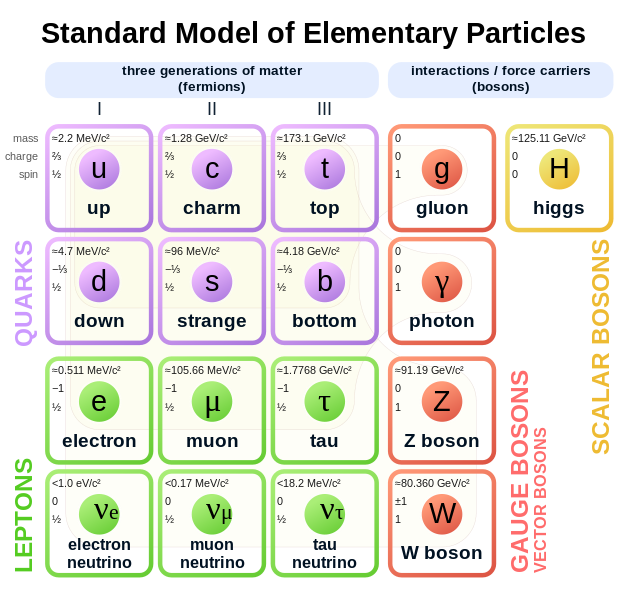
\includegraphics[width=\textwidth]{figures/intro/Standard_Model_of_Elementary_Particles.svg.png}
	\caption{
		The Standard Model of Particle Physics showing the twelve fermions and five bosons,
		their various properities (mass, charge, spin), labels (box and circle colors),
		and interactions (brown loops). Credit to Cush on wikipedia for
		providing this diagram freely accessible and usable for any purpose.
	}
	\label{fig:sm}
\end{figure}

The two lowest mass quarks -- the up and the down -- are the fundamental constituents of protons
and neutrons which make up the nuclei of atoms which make up all the day-to-day stuff we interact
with. These stay bound together within these nuclei via the strong nuclear force (mediated and
represented in \cref{fig:sm} by the gluon). These quarks and the top row of leptons also have an
electric charge enabling them to interact via with electromagnetic force.
The electromagnetic force, represented and mediated by the photon, is the force
responsible for light and magnetism. The lowest mass charged lepton (electron) is also very
abundant -- most commonly residing in orbits around nuclei helping form atoms. Both experiments in
this thesis utilize beams of electrons that have been accelerated to high energies and then
impinge upon a material of high density to initiate interactions for further study.

The mathematical expressions to calculate how these particles interact are complicated. As
mentioned earlier, physicists are lazy and so we have developed a method to represent the specifics
of these interactions without needing to write down any of the long mathematical formulae. These
representations are called ``Feynman diagrams'' after the 20th century physicist Richard Feynman.
Feynman diagrams allow us to represent interactions by defining a set of ``vertices'' that are
allowed by our theory and then constructing processes from these vertices that include the in- and
out- going particles that we wish to study. The further calculation of these diagrams is a defined
process that has been written into various computer programs (I say this to emphasize that these
diagrams directly represent the mathematics that can be used to calculate them).
\cref{fig:brem-feynman} shows an example Feynman diagram representing the bremsstrahlung process
where a charged lepton (\(\ell^-\)) interacts with a nucleus (\(Z\)) via a photon (\(\gamma\)) and
then emits another photon before recoiling. We can see three verticies in this diagram: two
``fundamental'' vertices where the lepton and photon lines connect and one ``effective'' vertex
where the photon connects with the nucleus. The fundamental vertices are actually strictly defined
within the Standard Model, but the effective vertex represents a helpful approximation that is
accurate at the energy scales we are studying.\footnote{ The distinction between fundamental and
	effective vertices is not a well defined one. I find it helpful here, but it is not necessarily
	made elsewhere in physics literature. }

\begin{figure}
	\centering
	\begin{tikzpicture}
		\begin{feynman}
			\vertex (in) {\(\ell^-\)};
			\vertex [right=of in] (nuc);
			\vertex [below=of nuc, blob] (nucleus) {\(Z\)};
			\vertex [right=of nuc, dot] (emit);
			\vertex [above right=of emit] (recoil) {\(\ell^-\)};
			\vertex [below right=of emit] (decay) {\(\gamma\)};
			\diagram*{
			(in) -- [fermion] (nuc) -- [fermion] (emit) -- [fermion] (recoil),
			(nucleus) -- [photon, edge label'=\(\gamma\)] (nuc),
			(emit) -- [photon] (decay),
			};
		\end{feynman}
	\end{tikzpicture}
	\caption{
		Feynman diagram for the bremsstrahlung process.
	}
	\label{fig:brem-feynman}
\end{figure}

Due to the complexity of the nucleus itself, the calculation of \cref{fig:brem-feynman} into
any observables is difficult to do without any approximations. However, one of the initial parametrizations of
bremsstrahlung offers a good glimpse of how it behaves \cite{bethe-heitler-1934}.
When doing experiments, we often count the number of particles produced with certain criteria.
These ``rates'' can then be translated into estimates of process cross sections (how likely a process
is to occur producing particles with the observed properties) with knowledge of
how the experiment was conducted. These cross sections are also calculatable from diagrams like
\cref{fig:brem-feynman} and the initial parameterization can be summarized as
\[
	\frac{d\sigma}{d E_\gamma} \propto \frac{1}{E_\gamma}
\]
This shows the dominant shape of the cross section
-- it grows as the energy of the produced photon
(\(E_\gamma\)) gets smaller. The full expression prevents the cross section from diverging as the
photon energy approaches zero; nevertheless, the general inverse relationship between the rate and
the energy of the produced photon holds in both the \ac{sm} calculations and observations from
experiments.\todo[citation]{need a citation for observation of bremsstrahlung photon energies?}
\cref{fig:recoil-electron-energy} shows another view of this rate: instead of looking at the
energy of the produced photon ($E_\gamma$), we can inspect the energy of the outgoing electron after
it emits the photon ($E_e$). This is more readily compared to other processes that do not
produce a photon and we can observe a large difference between this \ac{sm} process and other
possible processes that we search for.

\begin{figure}
	\centering
	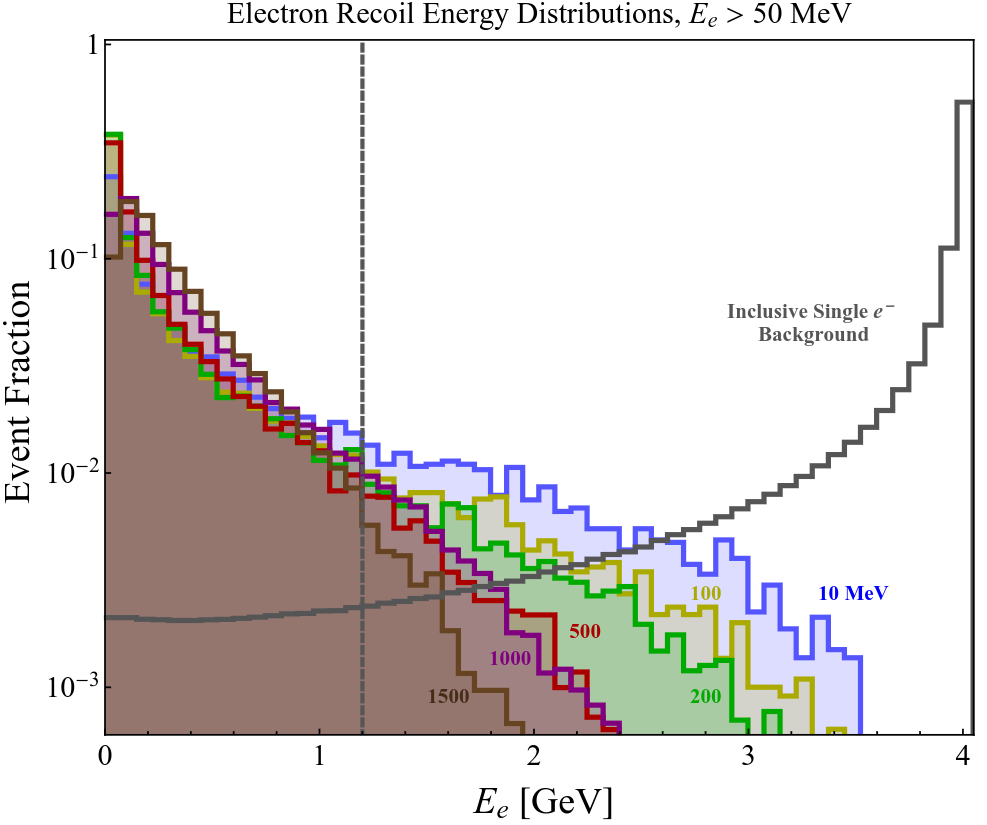
\includegraphics[width=0.5\textwidth]{figures/intro/photon-reject-fig-3-recoil-electron-energy.png}
	\caption{
		Energy of the outgoing electron ($E_e$) for standard processes (dominated by bremsstrahlung)
		in gray and some dark bremsstrahlung (see \cref{sec:dm:invisible}) in colors.
		Figure 3 from \cite{ldmx-photon-reject-2020}.
	}
	\label{fig:recoil-electron-energy}
\end{figure}

This inverse relationship is somewhat special and is mostly due to the fact that photons
do not have any mass; however, this special relationship opens a door towards potential
discovery. The vast majority of electrons interacting with a material will do so softly,
only emitting low energy photons, which distinctly separates these electrons from ones
that undergo rarer processes (or perhaps so-far undiscovered processes). Both experiments
described in this work make heavy use of this fact.\todo[more]{make sure to reference back
	to softness of sm brem in experiment sections.}

For the rest of this thesis, I intend to stay within this diagrammatic realm -- representing the theoretical
calculations being tested with these diagrams and limiting the scope of mathematical formulae
presented. Occasionally, the weight of these vertices which can be interpreted as the strength
of the interaction is presented along with the vertices in order to give a sense of scale
and connect these diagrams to the formulae that are included here.

\section{Standard Model Analogies}
The \ac{sm} has been extremely successful in describing the current world of particle physics,
including some intricate behaviors of particles that were incredibly confusing when first
encountered.
When attempting to describe unknown phenomena (\cref{chapter:dm}), we often draw on this
previous experience to form new ideas and models.
This section, while a brief detour, will help give context for two key behaviors that
the models we are searching for would give their particles.

\subsection{Particle Mixing}
All of the models tested for in this work use the idea of ``particle mixing'' in order
to connect the realm of theoretical/undiscovered particles with the realm of \ac{sm}
particles. In the quantum arena, we treat individual particles in a probabilistic
manner -- often times when we observe a particle with certain properties, it can
be observed again in a different context with different properties.
While this sounds odd, several experiments have supported this random nature
of the smallest particles over the course of twentieth century physics.
Specifically, kaons have been observed to ``swap'' with their own anti-particle,
which we can describe via this concept of mixing.

Kaons are particles that contain two quarks, one of which is a strange quark (or its
anti-quark). Describing kaons in this way allows us to mix neutral kaons with their
anti-particles, diagrammed in \cref{fig:kaon-box-diagram}. From a higher-level view,
where we are unaware of the constituents of the kaon, it appears like the neutral kaon (\(K_0\))
and its anti-particle (\(\overline{K}_0\)) are swapping places with some probability.
Our experiments can observe this probability by counting the frequency with which we
see \(K_0\) compared to \(\overline{K}_0\)\todo[citation]{Neutral kaon mixing citation}.
We can also use our model of the kaons (as composed of quarks) and calculate this
same probability (specifically, using the Feynman diagram shown in \cref{fig:kaon-box-diagram}).
Comparing the two gives us information about the \ac{sm} and how the quarks
interact with one another.

\begin{figure}
	\centering
	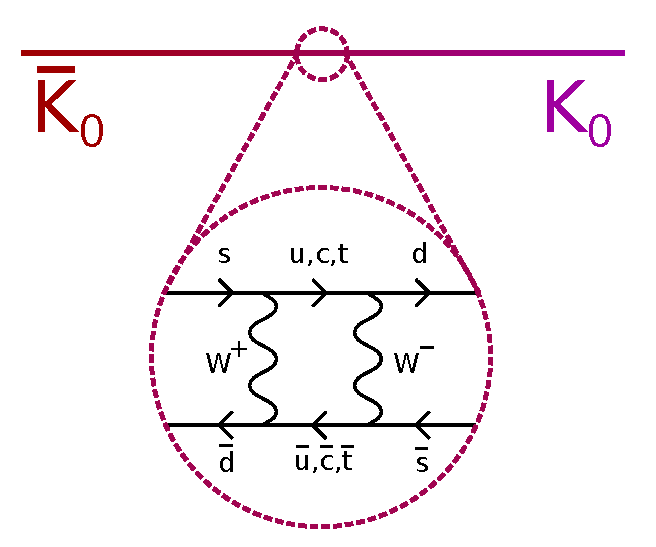
\includegraphics[width=0.5\textwidth]{figures/intro/Kaon-box-diagram-with-bar.pdf}
	\caption{
		Dipiction of neutral kaon and anti-kaon mixing including the underlying
		Feynman diagram that results from applying the \ac{sm} to this system.
		This figure was created by user
		\href{https://commons.wikimedia.org/wiki/File:Kaon-box-diagram-with-bar.svg}{NikNaks on Wikipedia}
		and is licensed under
		\href{https://creativecommons.org/licenses/by-sa/3.0/deed.en}{CC Attribution-Share Alike 3.0 Unported}.
	}
	\label{fig:kaon-box-diagram}
\end{figure}

\subsection{Displaced Particle Decays}
Ever since particle physicists have started designing detectors, we have also observed
particles that are ``missed'' by our detector mechanisms. \cref{fig:bubble-chamber}
shows an early example of this where a ``bubble chamber'' shows the paths of
charged particles passing through the liquid (the white lines). In the middle of this
image, you can observe two lines emerging seemingly out of nowhere (the red annotations were
added later).
The mechanism that allows a bubble chamber to observe the path of particles requires the particle
to have a charge, so a neutral particle (a \(\Lambda\) in this case) does not leave a path itself.
The only signal that it was there is the \emph{displaced vertex} from which two other particles
(probably a proton and a negative pion) emerge
(emphasized with a red circle in \cref{fig:bubble-chamber}).
This is a ``displaced decay'' of a particle which was produced by a high energy
(\qty{16}{\giga\electronvolt}) negative pion interacting with the liquid in the bubble chamber.

While particle physicists have developed other detector apparatuses, some of which can observe
neutral particles more directly, this more indirect detection mechanism is still extremely
useful especially if a model being tested has particles that have no way of directly interacting
with \ac{sm} matter (the stuff we make our detectors out of). \cref{part:hps} of this thesis
focuses entirely on an experiment designed to search for these displaced vertices, the displacment
of the vertex coming from the presence of an as-yet undiscovered particle being produced and then
decaying back into \ac{sm} particles.

\begin{figure}
	\centering
	\begin{tikzimage}[0.8\textwidth]{figures/intro/bubble-chamber.jpeg}
		% \draw[step=0.1,black,thin] (0.0,0.0) grid (1.0,1.0);
		\node (prod) at (0.4,0.54) {};
		\node[circle,draw=red] (decay) at (0.515,0.54) {};
		\draw[dashed,red,thick] (prod) -- (decay);

		\node (beam1) at (0.1,0.5) {\color{red}\(\pi^-\)};
		\node (beam2) at (0.2,0.5) {};
		\draw[->,red,thick] (beam1) -- (beam2);
	\end{tikzimage}
	\caption{
		Image of CERN's first liquid hydrogen bubble chamber from 1960 \cite{bubble-chamber-image-1960}
		with red annotations added. The red circle highlights the location described in the text where
		a \(\Lambda\) baryon decays into two particles (most likely a proton and a negative pion). The
		red dashed line traces out a possible path the \(\Lambda\) traveled before its decay.
	}
	\label{fig:bubble-chamber}
\end{figure}

\begin{todoenv}
	The Kaon system in the SM is rich with interesting physics and provides examples of specific
	physical phenomena that we can apply to our search for new physics.

	\begin{itemize}
		\item \(K_S\) 2-body decay is displaced by $O(3~\text{cm})$
	\end{itemize}

	Look into a kinetic mixing example from SM. Point out how particles can ``mix'' with one another
	in this quantum realm. Strong KM of photon (hadronix FF), maybe photon and Z mixing?
\end{todoenv}

%%%%%%%%%%%%%%%%%%%%%%%%%%%%%%%%%%%%%%%%%%%%%%%%%%%%%%%%%%%%%%%%%%%%%%%%%%%%%%%%
